%Präambel%
\documentclass[10pt]{scrartcl}
\usepackage[ngerman]{babel}
\usepackage[utf8]{inputenc}
\usepackage{graphicx}
\usepackage{amsmath}
\usepackage{amssymb}
\usepackage{multicol}
\usepackage{helvet}
\usepackage{lastpage}
\usepackage{geometry}
\usepackage{colortbl}
\usepackage{multirow}
\usepackage{color}
\usepackage{multicol}
\usepackage{wrapfig}
\makeatletter
\renewcommand*\env@matrix[1][*\c@MaxMatrixCols c]{%
  \hskip -\arraycolsep
  \let\@ifnextchar\new@ifnextchar
  \array{#1}}
\makeatother
\renewcommand{\familydefault}{\sfdefault}
%Kopfzeile%
\usepackage[headsepline, footsepline]{scrlayer-scrpage}
\pagestyle{scrheadings}
\clearpairofpagestyles
\setkomafont{pageheadfoot}{\normalfont\small}
\ihead{
\includegraphics[height=45pt]{images/HSRLOGO.jpg}}
\chead{}
\ohead{Zusammenfassung \\ Lineare Algebra}
\ifoot{Züger Raphael \\ B16}
\cfoot{\today}
\ofoot{\pagemark /\pageref{LastPage}}
%Seitengeometrie festlegen%
\geometry{left=20mm, right=15mm, top=30mm, bottom=15mm, includefoot=false, headsep = \dimexpr2\baselineskip-5mm\relax, footskip = \dimexpr1\baselineskip+4mm\relax,}
%Fusszeitenlinie höher setzen%
\ModifyLayer[addvoffset=-.8ex]{scrheadings.foot.above.line}
\ModifyLayer[addvoffset=-.8ex]{plain.scrheadings.foot.above.line}
\setcounter{tocdepth}{2}
\usepackage{booktabs}			% Schönere Tabellen
\usepackage{tabularx}			% Tabellen auf Seitenbreite
\usepackage{enumitem} 
\newlist{citemize}{itemize}{4} 
\setlist[citemize]{label=\textbullet ,nosep,topsep=-\parskip} 
%Tabellen///////////////////////////////////////////////////%
\newcolumntype{L}[1]{>{\raggedright\arraybackslash}p{#1}} % Tabelleninhalt linksausgerichtet
\newcolumntype{R}[1]{>{\raggedleft\arraybackslash}p{#1}} % Tabelleninhalt rechtsausgerichtet
\newcolumntype{C}[1]{>{\centering\arraybackslash}p{#1}} %  Tabelleninhalt zentriert
\setlength{\parindent}{0pt}
\setlength{\columnsep}{1cm}
\begin{document}
\section*{Zusammenfassung Lineare Algebra}
\begin{multicols}{2}
\subsubsection*{Definition Lineares Gleichungssystem LGS}
\begin{equation}
\begin{matrix}
a_{11}x_{1} & a_{12}x_{2} & \dots & a_{1n}x_{n} & = & b_{1} \\
a_{21}x_{1} & a_{22}x_{2} & \dots & a_{2n}x_{n} & = & b_{2} \\
& \vdots\\
a_{m1}x_{1} & a_{m2}x_{2} & \dots & a_{mn}x_{n} & = & b_{m} \\
\end{matrix}
\end{equation}
Wenn $ a_{ij} $ und $b{i}$ reelle Zahlen sind, dann ist es ein LGS.\\
$ a_{ij} $ = Koeffizienten\\
$ b = (b_{1} \dots b_{n}) $ = rechte Seite\\
$m$ = Anzahl Gleichungen\\
$n$ = Anzahl Variablen\\
Wenn m = n, nennt man das LGS quadratisch.\\
\subsubsection*{Matrixschreibweise}
\begin{equation}
\begin{pmatrix}[cccc|c]
a_{11} & a_{12} & \dots & a_{1n} & b_{1} \\
a_{21} & a_{22} & \dots & a_{2n} & b_{2} \\
& \vdots & & &\\
a_{m1} & a_{m2} & \dots & a_{mn} & b_{m} \\
\end{pmatrix}
\end{equation}
Mit der Linie und der rechten Seite nennt man diese Darstellung Erweiterte Koeffizientenmatrix.
\subsubsection*{Elementare Umformungen}
\begin{enumerate}
\item Vertauschen zweier Zeilen
\item Multiplizieren einer Zeile mit einer Zahl $\neq$ 0.
\item Addition einer Zeile auf eine andere Zeile
\end{enumerate}
\subsubsection*{Gauss-Jordan-Verfahren}
\par
Auch als Gauss-Algorithmus bekannt.
\begin{enumerate}
\item LGS in Erweiterter Koeffizientenmatrix schreiben: \begin{equation}
\begin{pmatrix}[cccc|c]
a_{11} & a_{12} & \dots & a_{1n} & b_{1} \\
a_{21} & a_{22} & \dots & a_{2n} & b_{2} \\
& \vdots & & &\\
a_{m1} & a_{m2} & \dots & a_{mn} & b_{m} \\
\end{pmatrix}
\end{equation}
\item Falls $a_{11} = 0$: Zeile vertauschen mit einer Zeile bei welcher der erste Koeffizient $\neq\neq$ 0 ist. (Oder Spalten vertauschen)
\item Erste Zeile mit $\dfrac{1}{a_{11}}$ multiplizieren so dass der erste Koeffizient = 1 wird.
\item Erste Zeile auf darauffolgende addieren, so dass jeweils erster Koeffizient 0 wird.
\item Mit zweiter Zeile analog Schritt 3 und 4 vorgehen. Daraus folgt eine Matrix in der Form:\begin{equation}
\begin{pmatrix}[ccc|c]
1 & a_{12}^{*} & a_{13}^{*} & b_{1}^{*} \\
0 & 1 & a_{23}^{*} & b_{2}^{*} \\
0 & 0 & 1 & b_{3}^{*} \\
\end{pmatrix}
\end{equation} 
\item Rückwärtseinsetzen: letzte Zeile auf obige Zeilen aufaddieren, so dass letzte Spalte = 0 wird.
\item Zweitletzte Zeile auf vorhergehende Zeilen aufaddieren, so dass zweitletzte Spalte = 0 wird usw. Daraus folgt eine Matrix in der Form:\begin{equation}
\begin{pmatrix}[ccc|c]
1 & 0 & 0 & b_{1}^{*} \\
0 & 1 & 0 & b_{2}^{*} \\
0 & 0 & 1 & b_{3}^{*} \\
\end{pmatrix}
\end{equation}
\item Lösung des LGS ablesen:\\  $x = b_{1}^{*}$ \\ $y = b_{2}^{*}$ \\ $z = b_{3}^{*}$\\ Dies entspricht dem Regulären Fall, das heisst dass das LGS eine exakte Lösung hat.
\end{enumerate}
\subsubsection*{Gauss-Verfahren: Singulärer Fall}
\begin{enumerate}
\item Keine Lösung: Wenn eine Zeile auf der linken Seite alles Nullen enthält und die rechte Seite $\neq$ 0 ist. Bsp.: \begin{equation}
\begin{pmatrix}[cc|c]
1 & 4 & 16 \\
0 & 0 & 24 \\
\end{pmatrix}
\end{equation}
\item Unendlich viele Lösungen: Lösungsanzahl $\neq$ Anzahl Variablen. Bsp.: \begin{equation}
\begin{pmatrix}[cc|c]
1 & 4 & 16 \\
0 & 0 & 0 \\
\end{pmatrix}
\end{equation}
Daraus folgt: $2x+y=16$ \\ und somit die Lösungsmenge: \begin{equation}\mathbb{L}=\left\lbrace \left( \begin{matrix} 0 \\ 16 \end{matrix}\right) + \lambda \left(\begin{matrix} 1 \\ -2 \end{matrix}\right)  \right | \lambda \in \mathbb{R} \rbrace  \end{equation}
\end{enumerate} 
\subsubsection*{Definition unabhängige Gleichungen} 
Widerspruchsfreie Gleichungen heissen unabhängig voneinander, wenn keine Gleichung weggelassen werden kann, ohne dass sich die Lösungsmenge verändert. \\ Der Gauss-Algorithmus eliminiert abhängige Gleichungen und reduziert das LGS auf unabhängige Gleichungen.
\subsubsection*{Rang des LGS}
Der Rang eines LGS ist definiert als die maximale Anzahl unabhängiger Gleichungen des LGS's.
\subsubsection*{Dimension der Lösungsmenge}
Ist das LGS lösbar, so ist die Dimension der Lösungsmenge = Anzahl Variablen n minus dem Rang des LGS. Bemerkungen:
\begin{enumerate}
\item Gibt es genauso viele unabhängige Gleichungen wie Variablen, so ist die Dimension der Lösungsmenge gleich Null.
\item Ist die Lösungsmenge leer ($\mathbb{L}=\left\lbrace \right \rbrace $), dann ist die Dimension nicht definiert.
\item Gibt es weniger unabhängige Gleichungen als Variablen und ist das LGS lösbar, so ist die Lösungsmenge unendlich. Die Dimension der Lösungsmenge ergibt sich aus der Differenz zwischen der Anzahl an Variablen n und der Anzahl unabhängiger Gleichungen.
\end{enumerate}
Wichtig: Die Dimension der Lösungsmenge und der
Rang eines LGS ist höchstens gleich der Anzahl an Variablen n.
\subsubsection*{Homogene LGS}
Ein LGS ist homogen, wenn die rechte Seite nur aus Nullen besteht:
\begin{equation}
\begin{matrix}
a_{11}x_{1} & a_{12}x_{2} & \dots & a_{1n}x_{n} & = & 0 \\
a_{21}x_{1} & a_{22}x_{2} & \dots & a_{2n}x_{n} & = & 0 \\
& \vdots &&&& \vdots\\
a_{m1}x_{1} & a_{m2}x_{2} & \dots & a_{mn}x_{n} & = & 0 \\
\end{matrix}
\end{equation}
Ist mindestens ein Eintrag auf der rechten Seite $\neq$ 0, dann ist das System inhomogen.\\
Ein homogenes LGS mit n Variablen besitzt eine Lösungsmenge der Dimension $n - r$, wobei r der Rang des LGS ist. Insbesondere besitzt es genau eine Lösung, wenn der Rang gleich n ist. Beispiel:\\
\begin{equation}
\begin{pmatrix}[ccc|c]
2 & 5 & 3 & 0 \\
6 & 7 & 5 & 0 \\
4 & 2 & 2 & 0 \\
\end{pmatrix} \Rightarrow \mathbb{L}^h=\left\lbrace \lambda\left( \begin{matrix} -1 \\ -2 \\ 4 \end{matrix}\right), \lambda \in \mathbb{R}  \right \rbrace 
\end{equation}
Die homogene Lösung ist immer ein Bestandteil der Lösung des inhomogenen LGS.
\subsubsection*{Vektoren}
Vektoren bestehen aus reellen Zahlen $x_{1} \dots x_{n}$. Angeordnet im Schema $x=\left( \begin{matrix} x_{1} \\ \vdots \\ x_{n}\end{matrix}\right) $ spricht man vom (reellen) (Spalten-)Vektor mit n Komponenten oder vom n-Dimensionalen Vektor. Die Menge dieser Vektoren wird mit $\mathbb{R}^{n}$ bezeichnet.\\
Als Nullvektor wird ein Vektor mit der folgenden Form bezeichnet: $0=\left( \begin{matrix} 0 \\ \vdots \\ 0\end{matrix}\right) $\\
Als i-ter Einheitsvektor $e_{i}$ wird ein Vektor bezeichnet, der an der i-ten Stelle den Eintag 1 hat und an allen anderen Stellen nur Nullen.
\subsubsection*{Rechenregeln Vektoren}
Summe:\\
\begin{equation}
x + y = \begin{pmatrix}
x_1\\
\vdots\\
x_n
\end{pmatrix} + \begin{pmatrix}
y_1\\
\vdots\\
y_n
\end{pmatrix} = \begin{pmatrix}
x_1 + y_1\\
\vdots\\
x_n + y_n
\end{pmatrix}
\end{equation}
Skalare Multiplikation:\\
\begin{equation}
\lambda \cdot x = \lambda \cdot \begin{pmatrix}
x_1 \\
\vdots \\
x_n
\end{pmatrix} = \begin{pmatrix}
\lambda \cdot x_1 \\
\vdots \\
\lambda \cdot x_n
\end{pmatrix}
\end{equation}
\subsubsection*{Lineare Abhängigkeit und Unabhängigkeit}
Linearkombination:
\begin{equation}
x = \lambda_1 \cdot v_1 + \dots + \lambda_k \cdot v_k = \sum_{i=1}^k \lambda_i \cdot v_i
\end{equation}
$v_1 \dots v_k$ sind Vektoren der Dimension n und $\lambda_1 \dots \lambda_k$ sind reelle Zahlen. Somit ist x eine Linearkombination der Vektoren $v_1 \dots v_k$.\\
Lineare Unabhängigkeit:\\ \\
Eine Menge Vektoren ($v_1 \dots v_k$) heissen Linear unabhängig, wenn die einzige Möglichkeit zur Linearkombination der Nullvektor ist:
\begin{equation}
0 = \lambda_1 \cdot v_1 + \dots + \lambda_k \cdot v_k = \sum_{i=1}^k \lambda_i \cdot v_i
\end{equation}
Lässt sich hingegen ein Vektor durch die anderen Vektoren darstellen, so sind diese abhängig voneinander. Enthält die Menge den Nullvektor, so ist die Menge per Definition linear abhängig.
\subsubsection*{Definition von Matrizen}
\begin{equation}
A = \begin{pmatrix}
a_{11} & a_{12} & \dots & a_{1n}\\
a_{21} & a_{22} & \dots & a_{2n}\\
\vdots & & \ddots & \vdots\\
a_{m1} & a_{m2} & \dots & a_{mn}
\end{pmatrix}
\end{equation}
A sei eine (reelle) Matrix mit m Zeilen und n Spalten. Man nennt sie deshalb ($m \times n$)-Matrix. Wenn m = n gilt, ist A eine Quadratische Matrix. Spezielle Formen sind:\\
a) Quadratische Matrix\\
b) (Spalten-) Vektoren($m \times 1$)-Matrix:
\begin{equation}
A= \begin{pmatrix}
a_{11}\\
\vdots\\
a_{m1}
\end{pmatrix}
\end{equation}
c) Zeilenvektoren ($1 \times n$)-Matrix:
\begin{equation}
A= \left(-1,0,4,5,10\right) 
\end{equation}
d) Nullmatrix:
\begin{equation}
A= \begin{pmatrix}
0 & 0 & 0\\
0 & 0 & 0 \\
\end{pmatrix}
\end{equation}
e) Diagonalmatrizen:
\begin{equation}
A= \begin{pmatrix}
8 & 0 & 0\\
0 & 1 & 0 \\
0 & 0 & -1
\end{pmatrix}, B= \begin{pmatrix}
1 & 3 & 8\\
0 & 4 & 12 \\
0 & 0 & -1
\end{pmatrix}, C= \begin{pmatrix}
1 & 0 & 0\\
0 & 4 & 0 \\
3 & 3 & -1
\end{pmatrix}
\end{equation}
A ist eine Diagonalmatrix, B eine obere Dreiecksmatrix und C eine untere Dreiecksmatrix.\\
f) Einheitsmatrix:\\
Alle Einträge sind Null bis auf die Diagonale, welche nur aus Einsen besteht:
\begin{equation}
I_n = I = \begin{pmatrix}
1 & 0 & \dots &  0\\
0 & 1 & \dots &  0 \\
\vdots & & \ddots & \vdots\\
0 & 0 & \dots & 1
\end{pmatrix}
\end{equation}
\subsubsection*{Rechenregeln Matrizen}
Wenn
\begin{equation}
A = \begin{pmatrix}
a_{11} & a_{12} & \dots & a_{1n}\\
a_{21} & a_{22} & \dots & a_{2n}\\
\vdots & & \ddots & \vdots\\
a_{m1} & a_{m2} & \dots & a_{mn}
\end{pmatrix}
\end{equation} und
\begin{equation}
B = \begin{pmatrix}
b_{11} & b_{12} & \dots & b_{1n}\\
b_{21} & b_{22} & \dots & b_{2n}\\
\vdots & & \ddots & \vdots\\
b_{m1} & b_{m2} & \dots & b_{mn}
\end{pmatrix}
\end{equation}
beliebige ($m \times n$)-Matrizen sind und $\lambda$ eine reelle Zahl ist, dann gelten die folgenden Gesetze:\\
Summe aus A und B:
\begin{equation}
A + B = \begin{pmatrix}
a_{11} + b_{11} & a_{12} + b_{12} & \dots & a_{1n} + b_{1n}\\
a_{21} + b_{21} & a_{22} + b_{22} & \dots & a_{2n} + b_{2n}\\
\vdots & & \ddots & \vdots\\
a_{m1} + b_{m1} & a_{m2} + b_{m2} & \dots & a_{mn} + b_{mn}
\end{pmatrix}
\end{equation}
Skalare Multiplikation der Matrix A mit $\lambda$:
\begin{equation}
\lambda \cdot A = \begin{pmatrix}
\lambda \cdot a_{11} & \lambda \cdot a_{12} & \dots & \lambda \cdot a_{1n}\\
\lambda \cdot a_{21} & \lambda \cdot a_{22} & \dots & \lambda \cdot a_{2n}\\
\vdots & & \ddots & \vdots\\
\lambda \cdot a_{m1} & \lambda \cdot a_{m2} & \dots & \lambda \cdot a_{mn}
\end{pmatrix}
\end{equation}
Multiplikation zweier Matrizen:\\
Damit zwei Matrizen multipliziert werden können, muss eine die Form $m \times k$ und die andere die Form $k \times m$ haben. Folgendes Beispiel zeigt das Vorgehen:
\begin{center}
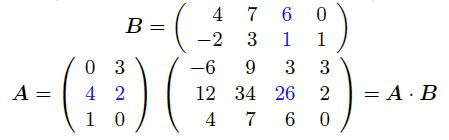
\includegraphics[scale=0.6]{images/falkscheanordnung.jpg}
\end{center}
Diese Merkregel nennt man Falk'sche Anordnung.\\
Achtung: $A \cdot B \neq B \cdot A$ !!
\subsubsection*{Transponierte und symmetrische Matrizen}
Transponieren heisst, Zeilen und Spalten vertauschen (aus einer ($m \times n$)- Matrix wird eine($n \times m$)- Matrix) :
\begin{equation}
A = \begin{pmatrix}
a_{11} & a_{12} & \dots & a_{1n}\\
a_{21} & a_{22} & \dots & a_{2n}\\
\vdots & & \ddots & \vdots\\
a_{m1} & a_{m2} & \dots & a_{mn}
\end{pmatrix}
\end{equation} somit ist die transponierte Matrix:
\begin{equation}
A^{T} = \begin{pmatrix}
a_{11} & a_{21} & \dots & a_{m1}\\
a_{12} & a_{22} & \dots & a_{m2}\\
\vdots & & \ddots & \vdots\\
a_{1n} & a_{2n} & \dots & a_{mn}
\end{pmatrix}
\end{equation}
Eine Matrix A ist symmetrisch wenn gilt:
\begin{equation}
A^{T} = A
\end{equation}
Somit gilt: eine symmetrische Matrix ist immer quadratisch.
\subsubsection*{Inverse und orthogonale Matrix}
Eine inverse Matrix muss immer quadratisch sein ($n \times n$). Wenn folgende Gleichung gilt, ist $A^{-1}$ die zu $A$ inverse Matrix:
\begin{equation}
A \cdot A^{-1} = A^{-1} \cdot A = I_n
\end{equation}
Eine Matrix A heisst orthogonal, wenn gilt:
\begin{equation}
A^{-1} = A^{T} \Rightarrow A\cdot A^{-1} = I \Leftrightarrow A \cdot A^{T} = I
\end{equation}
\subsubsection*{Rechenregeln für Matrizen}
Kommutativgesetz:\hfill $A + B = B + A$ \begin{flushright} $A \cdot B \neq B \cdot A$ \end{flushright}
Assoziativgesetz:\hfill $A+(B+C) = (A+B)+C$ \begin{flushright} $A \cdot (B \cdot C) = (A \cdot B) \cdot C$ \end{flushright}
Distributivgesetz:\hfill
$A \cdot (B+C) = A \cdot B + A \cdot C$ \begin{flushright} $(A+B) \cdot C = A \cdot C + B \cdot C$\end{flushright}
Skalare Multiplikation:\hfill
$(\lambda + \mu) \cdot A = \lambda \cdot A + \mu \cdot A$ \begin{flushright}
$(\lambda \cdot \mu) \cdot A = \lambda \cdot (\mu \cdot A)$\\
$\lambda \cdot (A+B) = \lambda \cdot A + \lambda \cdot B$ \\
$\lambda \cdot (A \cdot B) = (\lambda \cdot A) \cdot B = A \cdot (\lambda \cdot B)$\end{flushright}
Transponierte und inverse Matrizen:\hfill
$(A^T)^T = A$ \begin{flushright}
$(A \cdot B)^T = B^T \cdot A^T$ \\
$(A^{-1})^{-1} = A$ \\
$(A \cdot B)^{-1} = B^{-1} \cdot A^{-1}$\\
$(A^{-1})^T = (A^T)^{-1}$ \end{flushright}
\subsubsection*{Bild und Kern einer Matrix}
Der Kern oder Nullraum einer Matrix A ist wie folgt definiert:
\begin{equation}
ker(A) = \lbrace x \in \mathbb{R}^n | A \cdot x = 0 \rbrace
\end{equation}
und das Bild (Image) oder den Spaltenraum der Matrix A als:
\begin{equation}
im(A) = \lbrace b \in \mathbb{R}^m | \text{es gibt ein x mit } A \cdot x\end{equation}
\[= b \rbrace = \lbrace A \cdot x | x \in \mathbb{R}^n \rbrace\]

Beispiel: $A=\begin{pmatrix}1 & 4 & -2 \\ 1 & 4 & -2\end{pmatrix}$\\
Kern: homogenes LGS lösen:
\begin{equation}
\begin{pmatrix}[ccc|c]
1 & 4 & -2 & 0\\
0 & 0 & 0 & 0
\end{pmatrix} \Rightarrow \end{equation}
\[ker(A) = \left\lbrace  \lambda \left( \begin{matrix}
-4 \\ 1 \\ 0
\end{matrix} \right) + \mu \left(\begin{matrix}
2 \\ 0 \\ 1
\end{matrix} \right), \lambda,\mu \in \mathbb{R}  \right\rbrace\]
Für das Bild stellen wir die folgende Gleichung auf:
\begin{equation}
A \cdot x = \begin{pmatrix}
1 & 4 & -2 \\
1 & 4 & -2
\end{pmatrix} \cdot \begin{pmatrix}
x \\ y \\ z
\end{pmatrix} 
\end{equation}
\[= x \cdot \begin{pmatrix}
1 \\ 1
\end{pmatrix} + y \cdot \begin{pmatrix}
4 \\ 4 
\end{pmatrix} + z \cdot \begin{pmatrix}
-2 \\ -2
\end{pmatrix}\] \[= (x+4y-z) \cdot \begin{pmatrix}
1 \\ 1
\end{pmatrix} \Rightarrow\]
\[im(A) = \left\lbrace \lambda \cdot \begin{pmatrix}
1 \\ 1
\end{pmatrix}, \lambda \in \mathbb{R} \right\rbrace \]
\subsubsection*{Determinante}
Die Determinante einer ($n \times n$)-Matrix liefert die Lösbarkeit des LGS. Die Berechnung erfolgt mit dem Laplace'schen Entwicklungssatz nach der k-ten Spalte:
\begin{equation}
det(A) = |A| = \sum_{i=1}^n (-1)^{i+k} \cdot a_{ik} \cdot det(A_{ik})
\end{equation}
Für die Vorzeichen kann auf das folgende Schema verwendet werden:
\begin{equation}
\begin{pmatrix}
+ & - & + & - & \dots\\
- & + & - & + & \dots\\
+ & - & + & - & \dots\\
\vdots & \vdots & \vdots & \vdots & \ddots
\end{pmatrix}
\end{equation}
Dabei ist $A_{ik}$ die ($n-1 \times n-1$)-Matrix, welche aus A durch streichen der i-ten Zeile und der k-ten Spalte für die Entwicklung, entsteht.\\
Die Determinante einer ($2 \times 2$)-Matrix errechnet sich wie folgt:
\begin{equation}
det(A) = a_{11} \cdot a_{22} - a_{21} \cdot a_{12}
\end{equation}
und einer ($3 \times 3$)-Matrix:
\begin{equation}
det(A) = a_{11} \cdot a_{22} \cdot a_{33} + a_{12} \cdot a_{23} \cdot a_{31} + a_{13} \cdot a_{21} \cdot a_{32} \end{equation}
\[- a_{31} \cdot a_{22} \cdot a_{13} - a_{32} \cdot a_{23} \cdot a_{11} - a_{33} \cdot a_{21} \cdot a_{12}\]
\subsubsection*{Reguläre und singuläre Matrizen}
Sind alle Zeilenvektoren bzw. Spaltenvektoren von A linear unabhängig, so sagt man die Matrix A habe den vollen Rang. Vektoren sind dann von einander linear unabhängig wenn gilt $det(A)\neq0$.\\
Die Matrix $A$ besitzt nur dann eine Inverse Matrix $A^{-1}$ wenn sie den vollen Rang hat.\\
Eine Matrix A heisst regulär, wenn ihre Determinante ungleich Null ist. Sie ist somit singulär, wenn ihre Determinante gleich Null ist. Damit sind folgende Aussagen äquivalent:
\begin{itemize}
\item Die Matrix A ist regulär
\item Die Matrix A hat den vollen Rang
\item Die Zeilen- und Spaltenvektoren von A sind linear unabhängig
\item Die Matrix A besitzt die Inverse Matrix A\textsuperscript{-1}
\item $det(A)\neq0$
\end{itemize}
\subsubsection*{Determinanten von Diagonalmatrizen}
Die Determinante einer (oberen oder unteren) Dreiecksmatrix A ist gleich dem Produkt der Diagonalelemente: $det(A) = a_{11} \cdot a_{22} \cdot a_{nn}$
\subsubsection*{Rechenregeln mit Determinanten}
A und B sind beliebige ($n \times n$)-Matrizen und $\lambda$ eine reelle Zahl:\\
$det(\lambda \cdot A) = \lambda^n \cdot det(A)$\\
$det(A \cdot B) = det(A) \cdot det(B)$\\
$det(A) = det(A^T)$\\
Ist A zusätzlich eine reguläre Matrix gilt auch:\\
$det(A^{-1}) = \dfrac{1}{det(A)}$
\subsubsection*{Der Vektorraum $\mathbb{R}^2$}
Die Elemente des Vektorraumes sind Vektoren, welche aus zwei reellen Komponenten bestehen. Vektoren mit n Komponenten werden im Vektorraum $\mathbb{R}^n$ dargestellt. Damit es als Vektorraum gilt, müssen die Rechengesetze der Addition von Vektoren und der skalaren Multiplikation von Vektoren eingehalten sein.
\subsubsection*{Unterraum}
Ein Unterraum ist eine Teilmenge (U) eines Vektorraumes V. $U \in V$
\subsubsection*{Lineare Hülle, aufgespannter Raum}
M ist eine Menge von Vektoren im Vektorraum V.
\begin{equation}
H(M) = \left\lbrace\sum_{i=1}^k \lambda_i \cdot v_i | \lambda_1, \lambda_2, \dots \lambda_k \in\mathbb{R}\right\rbrace 
\end{equation}
H ist ein Unterraum von V, der als lineare Hülle von M bezeichnet wird oder als der von M aufgespannte Raum.
\subsubsection*{Erzeugendensystem}
Eine Menge von Vektoren E des Vektorraums V heisst Erzeugendensystem, wenn
\begin{equation}
H(M) = V
\end{equation}
Das heisst, dass jeder Vektor aus V durch eine Linearkombination aus E dargestellt werden.
\subsubsection*{Basis eines Vektorraums}
Eine Menge von Vektoren B des Vektorraumes V heisst Basis, wenn gilt:
\begin{itemize}
\item B ist ein Erzeugendensystem
\item B ist linear unabhängig
\end{itemize}
Die Dimension $dim(V)$ eines Vektorraums V ist definiert als die Anzahl der Basisvektoren einer Basis von V.
\subsubsection*{Kanonische Basis}
\begin{equation}
B = \left\lbrace e_1, e_2, \dots e_n\right\rbrace = \left\lbrace \begin{pmatrix}
1 \\ 0 \\ \vdots \\ 0
\end{pmatrix}, \begin{pmatrix}
0 \\ 1 \\ \vdots \\ 0
\end{pmatrix}, \dots, \begin{pmatrix}
0 \\ 0 \\ \vdots \\ 1
\end{pmatrix} \right\rbrace 
\end{equation}
heisst kanonische Basis oder Standardbasis des $\mathbb{R}^n$. Das heisst, dass $\mathbb{R}^n$ ein n-Dimensionaler Raum ist.
\subsubsection*{Skalarprodukt}
u und v sind Vektoren aus dem $\mathbb{R}^n$.
Dann ist das Skalarprodukt wie folgt definiert:
\begin{equation}
\langle u,v\rangle = u \bullet v = u^T \cdot v
\end{equation}
\[= u_1v_1 + u_2v_2 + \dots + u_nv_n = \sum_{i=1}^n u_iv_i\]
\subsubsection*{Betrag bzw. Norm}
v ist ein Vektor des $\mathbb{R}^n$. Dann ist die Länge des Vektors v =
\begin{equation}
\Vert v \Vert = \sqrt{\langle v,v \rangle} = \sqrt{v_1^2 + v_2^2 + \dots + v_n^2} = \sqrt{\sum_{i=1}^n v_i^2}
\end{equation}
\subsubsection*{Winkel zwischen zwei Vektoren}
u und v sind Vektoren aus dem $\mathbb{R}^n$. Der Winkel $\phi$ wird durch u und v eingeschlossen:
\begin{equation}
\cos (\phi) = \dfrac{\langle u,v \rangle}{\Vert u\Vert \Vert v \Vert}
\end{equation}
\subsubsection*{Orthogonal und Orthonormal}
u und v heissen orthogonal, wenn $\langle u,v \rangle = 0$ ist. \\
u und v heissen orthonormal, wenn $\langle u,v \rangle = 0$ und zusätzlich $\Vert u \Vert = \Vert v \Vert = 1$
\subsubsection*{Lineare Abbildung}
Eine Abbildung $l : U \rightarrow V$ vom Vektorraum U in den Vektorraum V heisst linear, wenn für alle Vektoren x und y aus U und alle reellen Zahlen $\lambda$ gilt:
\begin{equation}
l(x+y) = l(x) + l(y)
\end{equation}
\[l(\lambda x) = \lambda l (x)\]
Eine ($m \times n$)-Matrix A definiert eine Abbildung vom $\mathbb{R}^n$ in den $\mathbb{R}^m$.
\subsubsection*{Dimensionssatz}
A ist eine ($m \times n$)-Matrix der linearen Abbildung vom $\mathbb{R}^n$ in den $\mathbb{R}^m$. Die Dimension des Kerns (Nullraum) der Matrix A plus dem Bild der Matrix A ist gleich der Dimension des Vektorraums $\mathbb{R}^n$:
\begin{equation}
dim(im(A)) + dim(ker(A)) = n
\end{equation}
\subsubsection*{Eigenwertgleichung}
A ist eine ($n \times n$)-Matrix und x ein n-dimensionaler Vektor ungleich Null. Wenn
\begin{equation}
Ax = \lambda x , \lambda \in \mathbb{R}
\end{equation}
Dann nennt man den Vektor x einen Eigenvektor von A zum Eigenwert $\lambda$.
\subsubsection*{Charakteristisches Polynom}
A ist eine ($n \times n$)-Matrix. Man nennt das Polynom $det(A - \lambda I_n)$ vom Grad n in der Variable $\lambda$, das charakteristische Polynom von A.
\subsubsection*{Eigenwertzerlegung}
Zu jeder symmetrischen Matrix A, gibt es eine orthogonale Matrix U, mit $A=UDU^T$, wobei D eine Diagonalmatrix ist. Die Spalten von U sind  die Eigenvektoren von A und die Diagonalelemente von D sind die zugehörigen Eigenwerte.
\subsubsection*{Potenz einer Matrix}
$A^k = U D^k U^T$\\

\end{multicols}
\end{document}
